% AutoMLR (NeurIPS 2026) submission skeleton — swap \documentclass/preamble for the official Overleaf template before submitting.
% Part 1 (<=4 pages): agent-written research result. Part 2 (<=4 pages): human-written system account. Part 3 (<=1 page): reflections.
\documentclass[11pt]{article}
\usepackage[margin=1in]{geometry}\usepackage{graphicx,booktabs,amsmath,hyperref,xcolor}
\title{Do Discovered Exploration Procedures Generalize?\\An Autonomous Loop, the Harness Exploit It Found, and What Survives Replay}
\author{Andy Ye \\ University of Washington}
\begin{document}
\maketitle
\begin{abstract}
Exploration objectives for RL testers are designed by hand, and nobody knows whether the ones that reach some target states reach others. We let an
autonomous research loop discover an exploration \emph{procedure} --- code over a save/restore archive of simulator states --- on Kinetix, a suite of
2D physics games, scored on 337 planted defects with witness states, 30\% of levels and one whole defect class sealed from the search. The loop's first
answer was a procedure that beat every hand-designed and RL tester on every split. It was an exploit: a race in the vectorised archive let the
procedure restore physically impossible states, and every check that ran through the evaluator confirmed the gain. The one check that did not ---
reproducing each counted hit from a level reset --- caught it. On the fixed harness the discovered procedure is level with action-repeat random
(0.579 vs.\ 0.574 on the search split, 0.267 vs.\ 0.259 on the sealed class; 5 seeds). Re-run on the corrected harness, the search recovers: its new best is level with the strongest procedure from a parallel survey program and significantly ahead of every hand-designed and RL tester on the search split and the sealed class. We report what survives: a replay-verified benchmark with a
reachability calibration and a frozen protocol; a survey-driven program of 24 exploration procedures the loop then wrote and benchmarked, of which
nineteen beat action-repeat on the targets a single held input can reach (best 0.816 vs.\ 0.709) and the leader, split-and-pump, is ahead on the
exploration tier (0.440 / 50\% vs.\ 0.373 / 42\%) and on the full protocol beats every hand-designed, searched and RL tester on the search split (0.621 vs.\ 0.574) and the sealed class (0.338 vs.\ 0.259; paired $+0.079\pm0.035$); the finding that the exploration tier's residual is a barrier common to all 24 procedures (their union
reaches 24 of 43 targets against the best single procedure's 22, and 36 of the 37 never-reached targets have never been witnessed by any method); and
bounds on the practical value of any of it: PPO overtakes the procedures at $4\times$ the budget, the procedures find targets 5--9$\times$ cheaper, and
nothing transfers across engines. Twenty-eight replay-verified engine anomalies (seven severity-A, including four joint tears) on shipped and generated levels come from the same runs. The benchmark, the
procedures and Part~1 were produced by the loop; the authors built and verified the oracles and document every intervention, including the exploit.
\end{abstract}

\section*{Part 1 --- Auto research result (agent-written)}
% AGENT-WRITTEN (Claude, this session), post-reset version. Every number is regenerated by a script from logs on the FIXED harness
% (one archive writer per slot; every counted hit replays through the harness).
% Tables: table_transfer_fixed (scripts/make_tables.py), table_methods (scripts/methods_table.py), table_cost (scripts/cost_table.py),
% table_breadth (scripts/breadth_table.py), table_bugs (scripts/update_bugs.sh). Superseded exploit-era files: part1.tex, table_transfer.tex,
% table_feasibility.tex.

\subsection*{1.1 The argument}
Exploration objectives for game testers are hand-designed, and where they have been evaluated as testers the record is poor: random beats RND asymptotically in
large maps~\cite{goexplore-reach}, more search made MCTS worse at reaching faults~\cite{ariyurek-mcts}, and coverage anti-correlates with bugs
found~\cite{ccpt}. We set an autonomous loop the task of discovering the exploration \emph{procedure} itself --- code over a save/restore archive of simulator
states~\cite{goexplore} --- and asked the workshop's question: does what it discovers generalize? The project's answer is one sentence: \textbf{a discovered
tester generalizes exactly as far as the evaluator it was optimized against --- the search is interchangeable, the fitness is the steering wheel.} Part~1
establishes that claim six ways, each a contribution on its own: an evaluator worth steering by (the benchmark, \S1.2); what an untrusted evaluator steers into
(the exploit, \S1.3); what a well-aimed one beats (every baseline at equal budget, \S1.4, and the cost curve, \S1.6); how headroom placement, not search effort,
produces advances (runs 9--12, \S1.3, \S1.5, \S1.8); how evaluator breadth buys engine-generality twice over (\S1.6); and the object-level payoff of steering
well --- 28 replay-verified real anomalies (\S1.7). The composition negatives (\S1.8) close the argument from the other side: nothing you do to \emph{finished}
programs substitutes for changing what they were optimized against.

\subsection*{1.2 Setup}
\textbf{Targets.} Kinetix~\cite{kinetix} 2D physics levels (74 shipped; 64 freshly generated ones for a second suite). A target is a
planted defect with a programmatic witness state: a boundary wall removed (OOB; a moving shape leaves the arena), an obstacle made
non-solid (TUNNEL; a collidable body's centroid inside it), a neutral shape given the goal role (SHORTCUT), restitution raised
(ANOMALY; speed above a per-level threshold), a hazard made harmless (DISARMED). 337 instances on the shipped levels (K-Defect) and 452 on the
generated ones (K-Fresh); a level-win suite (K-Goal, 52/22 targets) uses the unmodified win condition. \textbf{Exclusions.} Instances that are
unwitnessable by construction (the collision matrix forbids every dynamic body from touching the target: 5 TUNNEL instances) or witnessed by
doing nothing are dropped from every denominator (search 127 $\to$ 119, held-out levels 59 $\to$ 58, held-out class 148); the counts are
stated in each caption. \textbf{Tiers.} A constant-input probe (each of the 11 actions held from reset for 256 steps) sorts targets into a
\emph{constant-input tier} (a single held input witnesses it; 42 of the search targets) and an \emph{exploration tier} (77 search, 12 held-out-level
and 16 held-out-class targets in the bench subsets). \textbf{Procedures.} A procedure drives $B$ workers through \texttt{init/restore/act/archive}
hooks over $K$ archived simulator states, in pure JAX; hand-designed baselines are uniform random, action-repeat random (sticky
actions) and a Go-Explore-style archive (SimHash cells, restores $\propto 1/\sqrt{\text{visits}}$); RL testers are PPO with count,
RND, ICM, curiosity-proximity and task objectives. \textbf{Metric.} $1-\min(\text{steps},\text{budget})/\text{budget}$ to the first witness
(0 if never), averaged over instances and seeds, and the fraction witnessed. \textbf{Protocol} (frozen; hash \texttt{7459c8de2a51}): levels 70/30
by hash order; OOB held out of every fitness; fitness seeds 0--2 at $128\times1024$ steps; evaluation seeds 100--104 at $128\times2048$.
\textbf{Verification.} Every first hit records its worker's action chain back to the level reset in an append-only lineage log and is
re-simulated through the harness at the run's own lane count before it counts; unreproduced hits are scored as misses (on the GPU none were; on the CPU bench the level-batch dimension changes the physics numerics enough that one hit in about a hundred rows fails to replay and is dropped). Real-anomaly
oracles on clean levels (left the arena, inside a static solid, joint torn, runaway speed or NaN) use per-level thresholds calibrated on
random play and persistence rules. \textbf{Prior work.} PhyFu~\cite{phyfu} fuzzes physics engines (including Brax) with physics-law
oracles on micro-scenarios; injected-fault testing scores recall at an interaction budget~\cite{ariyurek-mcts,gbqa}; meta-learned
curiosity~\cite{alet} searched over exploration algorithms on control tasks without a target benchmark or a held-out class. Ours is scored
like injected-fault testing, reads simulator state, seals splits by level \emph{and} by class, and reproduces every counted hit.

\subsection*{1.3 The search, and the exploit it found}
ShinkaEvolve~\cite{shinka} evolved the procedure from the Go-Explore seed (Sonnet~5 / Opus~5 proposing patches; fitness on the search split).
Run~1's best program reached a fitness of 0.699 against the seed's 0.629 and appeared to transfer: 0.666 / 0.617 / 0.418 on search / held-out
levels / held-out class against 0.566 / 0.575 / 0.266 for action-repeat random (5 seeds). Its mechanism was two archive pools that keep the
fastest and the most goal-proximate states and restore from them constantly. When several vectorised workers wrote the same slot in one step,
the state, feature and lineage scatters disagreed on the GPU, and the slot held a \emph{chimera} --- one world's positions with another's
velocities --- whose next step is violent enough to fire OOB, ANOMALY and TUNNEL witnesses. The fitness rewarded it, the transfer test
passed it (chimeras work on every level and class), and the ablations confirmed it, because all of them ran on the same evaluator. It was
caught by the rule that a reported anomaly must replay from reset: chains reconstructed from the lineage log replayed 12 of 86 flagged
runs. A lineage audit found 13 of 64 archived states inconsistent with their own chains (0 of 64 and 0 of 96 after the fix), and a GPU
audit measured the mechanism directly: 24\% and 7\% of the program's archived states on two instances were chimeras under the legacy
race and none under the fix. On the fixed harness the same program scores 0.579 / 0.566 / 0.267 (Table~\ref{tab:transfer_fixed}), level with
action-repeat random (paired per-instance gain $+0.006\pm0.039$ / $-0.023\pm0.033$ / $+0.008\pm0.036$, 95\% CIs over instances --- no significant gain on any split); the run-9 search restarted from the seed on the fixed harness moved 0.510 $\to$ 0.588 in fitness, and its best program scores 0.613 / 0.583 / 0.344 on the full protocol --- paired gains over action-repeat of $+0.039\pm0.035$ (search) and $+0.085\pm0.038$ (sealed class), both instance-significant, and statistically indistinguishable from the strongest survey procedure on every split (\S1.4). The loop that was fooled by its own evaluator finds a real procedure once the evaluator is sound; run 10, with the replay built into the fitness itself and the strongest known procedure (split-and-pump) as its seed, finished 40 generations without beating that seed (best = generation 0; 15 of 41 candidates failed outright): from a weak seed the sound-evaluator search climbs to the survey frontier, and from the frontier it does not exceed it. Run 11, with the 24 reachable-hard targets (plus the easy bench) as fitness, moved 0.783 $\to$ 0.792 and its best transfers as a small but instance-significant search-split gain over split-and-pump ($+0.011\pm0.009$, bootstrap $[+0.004,+0.021]$; ties on the other splits) --- the one improvement over the frontier any method achieved, bought by pointing the fitness at the tier where procedures differ. Run 12 added regret normalization and paired-$\Delta$ selection to that fitness and produced a \emph{trade} rather than an advance: significantly better on the sealed class ($+0.015$, bootstrap $[+0.003,+0.030]$) and significantly worse on search ($-0.012$, $[-0.025,-0.001]$) than run 11 --- shaped fitness moves where a program sits on the search--transfer frontier; expanding the frontier itself found its answer in run 13, a multi-engine regret search seeded from run 11's best: its program statistically ties run 11 on every Kinetix split ($-0.006\pm0.007$ / $+0.003\pm0.005$ / $-0.000\pm0.006$ paired) while adding partial transfer to five engine families outside its fitness --- the first program that is simultaneously at the Kinetix frontier and usable off-engine.

\subsection*{1.4 Result 1 --- what actually reaches the targets}
\begin{table}[t]\centering\small
\begin{tabular}{lccc}
\toprule
Tester & Search & Held-out levels & Held-out class (OOB) \\
\midrule
Random & 0.456$\pm$0.006 (49\%) & 0.539$\pm$0.008 (56\%) & 0.105$\pm$0.006 (12\%) \\
Action-repeat random & 0.574$\pm$0.007 (60\%) & 0.589$\pm$0.002 (60\%) & 0.259$\pm$0.008 (29\%) \\
Go-Explore (seed) & 0.540$\pm$0.004 (57\%) & 0.566$\pm$0.007 (59\%) & 0.220$\pm$0.011 (27\%) \\
\midrule
Split-and-pump (survey) & 0.621$\pm$0.004 (66\%) & 0.590$\pm$0.003 (61\%) & 0.338$\pm$0.005 (37\%) \\
Actuator saturation (survey) & 0.622$\pm$0.003 (65\%) & 0.590$\pm$0.012 (61\%) & 0.330$\pm$0.008 (38\%) \\
Velocity maximisation (survey) & 0.603$\pm$0.003 (64\%) & 0.596$\pm$0.003 (62\%) & 0.333$\pm$0.004 (37\%) \\
Root CEM (survey) & 0.594$\pm$0.004 (63\%) & 0.584$\pm$0.003 (60\%) & 0.278$\pm$0.011 (32\%) \\
Death-aware checkpoints (survey) & 0.590$\pm$0.005 (63\%) & 0.591$\pm$0.003 (61\%) & 0.267$\pm$0.006 (30\%) \\
Resonance sweep (survey) & 0.587$\pm$0.013 (63\%) & 0.548$\pm$0.013 (57\%) & 0.276$\pm$0.005 (30\%) \\
\midrule
Searched: hard-tier fitness (run 11) & 0.632$\pm$0.003 (66\%) & 0.595$\pm$0.007 (61\%) & 0.327$\pm$0.005 (36\%) \\
Searched: fixed harness (run 9) & 0.613$\pm$0.007 (64\%) & 0.583$\pm$0.007 (61\%) & 0.344$\pm$0.007 (38\%) \\
Searched: racy era (run 1) & 0.579$\pm$0.007 (63\%) & 0.566$\pm$0.006 (59\%) & 0.267$\pm$0.010 (31\%) \\
\midrule
Opus design: pair-ladder & 0.600$\pm$0.009 (64\%) & 0.582$\pm$0.003 (60\%) & 0.300$\pm$0.007 (33\%) \\
Opus design: macrosweep & 0.600$\pm$0.003 (63\%) & 0.575$\pm$0.003 (60\%) & 0.294$\pm$0.008 (33\%) \\
Opus design: elites & 0.595$\pm$0.007 (62\%) & 0.579$\pm$0.003 (60\%) & 0.318$\pm$0.009 (34\%) \\
\midrule
PPO+count & 0.487$\pm$0.017 (56\%) & 0.538$\pm$0.007 (58\%) & 0.184$\pm$0.014 (27\%) \\
PPO+curiosity-proximity & 0.492$\pm$0.014 (57\%) & 0.535$\pm$0.005 (57\%) & 0.179$\pm$0.016 (26\%) \\
PPO+task & 0.481$\pm$0.033 (54\%) & 0.510$\pm$0.025 (55\%) & 0.161$\pm$0.003 (23\%) \\
PPO+RND & 0.461$\pm$0.019 (51\%) & 0.502$\pm$0.017 (55\%) & 0.124$\pm$0.016 (17\%) \\
PPO+ICM & 0.451$\pm$0.028 (50\%) & 0.491$\pm$0.011 (52\%) & 0.117$\pm$0.019 (16\%) \\
\bottomrule
\end{tabular}
\caption{Score $=1-\min(\text{steps},\text{budget})/\text{budget}$ (mean $\pm$ 95\% CI over 5 seeds) and fraction of planted defects witnessed, per split; budget $128\times2048$ env steps per instance; size-l configuration, 74 shipped levels. Instances unwitnessable by construction or witnessed by no-ops alone are excluded from the denominators (0 of 148, 8 of 127, 1 of 59).Fixed harness; program rows evaluation seeds 100--104, PPO rows training seeds 0--2. Run 11 (reachable-hard fitness) holds the only instance-significant gain over split-and-pump (search $+0.011\pm0.009$); run 9 searched from the Go-Explore seed.}
\label{tab:transfer_fixed}
\end{table}
\begin{table}[t]\centering\small\setlength{\tabcolsep}{4pt}
\begin{tabular}{llrrrrr}\toprule
 & & \multicolumn{2}{c}{Constant-input tier (48)} & \multicolumn{3}{c}{Exploration tier (43/12/16)} \\
\cmidrule(lr){3-4}\cmidrule(lr){5-7}
Procedure & family & search & sealed cls & search & held-out lvl & sealed cls \\ \midrule
Split-and-pump & hybrid & 0.807\,/\,86 & 33 & 0.440\,/\,50 & 38 & 19 \\
Actuator saturation & coherence & 0.816\,/\,88 & 33 & 0.407\,/\,49 & 29 & 22 \\
Velocity-aligned drive & energy & 0.755\,/\,82 & 33 & 0.395\,/\,44 & 33 & 28 \\
Velocity maximisation & energy & 0.766\,/\,83 & 31 & 0.391\,/\,47 & 29 & 25 \\
Split-and-pump + velocity & hybrid$^2$ & -- & -- & 0.391\,/\,45 & 33 & 25 \\
KPIECE archive & planning & 0.750\,/\,82 & 28 & 0.384\,/\,44 & 38 & 22 \\
Death-aware checkpointing & termination & 0.772\,/\,86 & 25 & 0.379\,/\,43 & 33 & 9 \\
Macrosweep (LLM design) & baseline & 0.751\,/\,81 & 25 & 0.376\,/\,43 & 25 & 25 \\
Learned effects + steering & planning & 0.749\,/\,81 & 31 & 0.374\,/\,43 & 42 & 25 \\
Pair-ladder (LLM design) & baseline & 0.724\,/\,79 & 28 & 0.374\,/\,42 & 33 & 16 \\
Contact branching & contact & 0.730\,/\,82 & 25 & 0.373\,/\,43 & 29 & 22 \\
Action-repeat random (hand-designed) & baseline & 0.709\,/\,75 & 25 & 0.373\,/\,42 & 33 & 16 \\
Directed power schedule & fuzzing & 0.753\,/\,82 & 25 & 0.373\,/\,43 & 33 & 16 \\
CEM over plans & optimisation & 0.761\,/\,83 & 25 & 0.369\,/\,42 & 33 & 22 \\
Go-Explore + PLR & hybrid & 0.732\,/\,82 & 25 & 0.367\,/\,42 & 33 & 22 \\
Root CEM & optimisation & 0.806\,/\,88 & 28 & 0.356\,/\,42 & 33 & 22 \\
Root CEM + ratchet & hybrid$^2$ & -- & -- & 0.354\,/\,41 & 33 & 19 \\
UCB tree & planning & 0.720\,/\,81 & 19 & 0.351\,/\,40 & 33 & 19 \\
$\zeta$-greedy holds & coherence & 0.764\,/\,82 & 22 & 0.343\,/\,40 & 33 & 22 \\
Rare-event splitting & rare-event & 0.764\,/\,83 & 25 & 0.342\,/\,40 & 33 & 16 \\
MAP-Elites & QD & 0.740\,/\,82 & 31 & 0.339\,/\,40 & 33 & 19 \\
Resonance sweep & energy & 0.771\,/\,83 & 28 & 0.337\,/\,40 & 29 & 16 \\
Run-1 program (exploit era) & baseline & 0.707\,/\,81 & 25 & 0.336\,/\,40 & 25 & 22 \\
Go-Explore + yield credit & hybrid & 0.670\,/\,79 & 25 & 0.318\,/\,38 & 33 & 9 \\
Go-Explore + $\zeta$ & hybrid & 0.652\,/\,75 & 25 & 0.307\,/\,38 & 33 & 9 \\
Go-Explore seed & baseline & 0.639\,/\,72 & 22 & 0.300\,/\,34 & 29 & 12 \\
\bottomrule\end{tabular}
\caption{Exploration procedures on the method bench (fixed harness; every counted hit replays through the harness). Constant-input tier: the stratified 48-target subset of the size-l splits (128$\times$1024 steps, seeds 100,101,102); exploration tier: the 43 / 12 / 16 targets no held input reaches (128$\times$1024, seeds 100,101). Cells: score\,/\,\% detected (score $=1-\text{first hit}/\text{budget}$, 0 when missed); sealed-class and held-out-level cells give \% detected. Sorted by exploration-tier search score. On the exploration tier the union over all procedures reaches 24/43 search targets against the best single procedure's 22: the residual is a common barrier (\S\ref{sec:barrier}).}
\label{tab:methods}\end{table}

With the loop's own candidate gone, the agent surveyed four literatures (sampling-based motion planning and rare-event simulation;
falsification and fuzzing; exploration priors and quality-diversity; game-QA heuristics), diagnosed the 149 missed targets, and wrote 24
procedures as hooks programs, each benchmarked on a stratified 48-target subset of the constant-input tier and on the exploration tier
(Table~\ref{tab:methods}). The diagnosis fixed the design brief: a single held input witnesses 38 of the 55 targets action-repeat finds
fastest and none of the 149 it misses; the misses need coherent inputs for 20--180 steps, survival past episode terminations (maze levels
kill every held input within $\sim$15 steps; driving levels win and reset at $\sim$200), or an energy ladder no single hold climbs.
\textbf{Constant-input tier.} Nineteen of the 23 other procedures beat action-repeat random (0.709 / 75\%); the leaders --- actuator saturation 0.816 / 88\%,
split-and-pump 0.807 / 86\%, root CEM 0.806 / 88\% --- gain 0.10 in score and 11--13 points of detection, and the Go-Explore seed the
search started from is last but one (0.639). \textbf{Exploration tier.} The field compresses: split-and-pump leads at 0.440 / 50\% against
action-repeat's 0.373 / 42\%, with saturation (0.407 / 49\%), velocity-aligned drive, velocity maximisation, KPIECE and death-aware
checkpointing between them; on the sealed class the velocity/steering family leads (velocity-aligned 28\%, velocity-max and steering
25\%, action-repeat 16\%). The two hybrids of the leaders do not beat their parents. \textbf{Full protocol.} Table~\ref{tab:transfer_fixed} re-evaluates the leading procedures on all three splits at $128\times2048$, five seeds: split-and-pump reaches 0.621 (66\%) on the search split, 0.590 (61\%) on held-out levels and 0.338 (37\%) on the sealed class --- the best figures of any tester on the first and third split --- with paired per-instance gains over action-repeat of $+0.047\pm0.037$ (bootstrap $[+0.013,+0.086]$) and $+0.079\pm0.035$ (bootstrap $[+0.047,+0.114]$; better on 21\% of instances, worse on 1\%): both instance-significant. Velocity maximisation is significant on the same two splits (0.603 / 0.596 / 0.333; sealed gain $+0.074\pm0.035$); root CEM is not ($+0.020\pm0.030$, $+0.019\pm0.022$); held-out levels remain a tie for every tester ($\le$0.596 vs.\ 0.589). Saturation matches them (0.622 / 0.590 / 0.330; paired vs.\ action-repeat $+0.048\pm0.038$ and $+0.071\pm0.037$, both significant; vs.\ split-and-pump $+0.001$ and $-0.008$, indistinguishable), so the top of the field is a statistical tie of three survey procedures and the run-9 searched program; death-aware checkpointing (0.585 / 0.581 / 0.267) and resonance (0.582 / 0.539 / 0.276) sit with the earlier designs. Among the earlier hand-written designs, pair-ladder (0.600 / 0.582 / 0.300)
and macrosweep (0.600 / 0.575 / 0.294) are the best; pair-ladder's gain over action-repeat on the sealed class is instance-significant ($+0.041\pm0.032$; bootstrap $[+0.010, +0.072]$; better on 16\% of instances, worse on 3\%) and its search-split gain is not ($+0.026\pm0.031$).

\subsection*{1.5 Result 2 --- the hard tier is a common barrier}
\label{sec:barrier}
The natural next step, a portfolio of the leaders, would not help. On the exploration-tier bench the union over all 24 procedures reaches
24 of 43 search targets against the best single procedure's 22 --- a greedy portfolio adds one target from KPIECE and one from velocity-aligned
drive and nothing else --- and on held-out levels and the sealed class the union equals the best single procedure (5 of 12, 5 of 16). Nineteen
search targets (9 SHORTCUT, 6 ANOMALY, 4 DISARMED), seven held-out-level and eleven sealed-class targets are reached by nobody, and 36 of those
37 have never been witnessed by any valid tester at any budget we have run. Restarting inside one budget does not help either: four restarts
change action-repeat's and the discovered program's scores by less than 0.005 on every split, so the misses are structural, not seed-unlucky.
Restricted to the targets some procedure does reach, the ranking is a ranking of speed: split-and-pump 0.789 / 90\% against action-repeat's
0.669 / 75\% on the 24 reachable-hard search targets. The diagnosis's automated blocker labels flag none of the 37, but its records show what they demand: six are ANOMALY targets that need 12\,m/s from a motor-only or weak-thrust agent, seven need a wheeled or jointed motor-only agent to climb 0.5--4.5\,m, twelve need a thruster with thrust-to-weight 0.4--1.0 to traverse 0.6--4.2\,m past three to five live hazards with 15--40-step holds, and the oracle-guided probe that is told the witness location reached none of them. The empirical answer is now in: at 4$\times$ the budget with five seeds, the six leading procedures reach \emph{one} of the 37 (an actuator-saturation hit on one search target); the other 36 are excluded as unwitnessable at $4\times$ budget. On the witnessable exploration tier the picture sharpens: 25 of 43 search targets are witnessable and split-and-pump reaches 22 of them (88\%; velocity family and saturation 84\%), and the witnessable held-out-level and sealed-class subsets (5 and 5) are fully covered by several procedures.
A per-class view says what the frontier is: SHORTCUT is the class no procedure moves (union 25\%, equal to action-repeat) even with the
mechanism the diagnosis prescribed for it (driving every motor to its stop), and run 11 made that fitness its signal and produced the one significant gain over the frontier (\S1.3).

\subsection*{1.6 Result 3 --- RL testers, cost, and breadth}
\begin{table}[t]\centering\footnotesize
\begin{tabular}{lrrrrrr}
\toprule
Tester & \multicolumn{2}{c}{Search (common $n$=60)} & \multicolumn{2}{c}{Held-out levels (common $n$=30)} & \multicolumn{2}{c}{Held-out class (common $n$=21)} \\
 & median steps & found & median steps & found & median steps & found \\
\midrule
Action-repeat random & 3.8k & 60\% & 3.3k & 59\% & 5.2k & 29\% \\
Go-Explore (seed) & 4.2k & 57\% & 3.3k & 58\% & 6.0k & 27\% \\
Discovered (run 1 best) & 3.8k & 62\% & 3.3k & 58\% & 7.5k & 31\% \\
Opus: pair-ladder & 3.7k & 63\% & 3.3k & 59\% & 4.9k & 33\% \\
PPO+count & 5.2k & 56\% & 4.2k & 57\% & 45.1k & 27\% \\
PPO+RND & 5.2k & 51\% & 4.2k & 54\% & 23.9k & 17\% \\
\bottomrule
\end{tabular}
\caption{Cost per target: median simulator steps to the first witness over the instances every compared tester finds, and the fraction of all instances found, per split (5 seeds; RL testers 3 seeds).}
\label{tab:cost}
\end{table}

\begin{table}[t]\centering\footnotesize
\begin{tabular}{lccccccccccc}
\toprule
Suite / split & Random & Action-repeat & Go-Explore & Split-and-pump & Saturation & Searched multi-engine (run 7) & Searched multi-engine x regret (run 13) & Searched run 1 & Opus macrosweep & PPO+count & PPO+RND \\
\midrule
K-Defect / srch (n=119) & 49$\pm$1 & 60$\pm$0 & 57$\pm$0 & 66$\pm$1 & -- & -- & -- & 63$\pm$1 & 63$\pm$1 & 56$\pm$2 & 51$\pm$0 \\
K-Defect / h-lvl (n=58) & 56$\pm$1 & 60$\pm$0 & 59$\pm$1 & 61$\pm$1 & -- & -- & -- & 59$\pm$2 & 60$\pm$1 & 58$\pm$3 & 55$\pm$0 \\
K-Defect / h-cls (n=148) & 12$\pm$1 & 29$\pm$1 & 27$\pm$1 & 37$\pm$1 & -- & -- & -- & 31$\pm$1 & 33$\pm$1 & 27$\pm$2 & 17$\pm$2 \\
K-Goal / srch (n=52) & 36$\pm$3 & 58$\pm$1 & 53$\pm$2 & -- & -- & -- & -- & 59$\pm$2 & 67$\pm$2 & 52$\pm$6 & 38$\pm$3 \\
K-Goal / h-lvl (n=22) & 29$\pm$2 & 82$\pm$3 & 71$\pm$6 & -- & -- & -- & -- & 81$\pm$3 & 76$\pm$3 & 65$\pm$3 & 38$\pm$3 \\
K-Fresh / srch (n=444) & 30$\pm$1 & 37$\pm$1 & 35$\pm$0 & 41$\pm$0 & 43$\pm$0 & -- & -- & 40$\pm$1 & -- & -- & -- \\
G-MountainCar / srch (n=6) & 0$\pm$0 & 100$\pm$0 & 67$\pm$15 & 100$\pm$0 & 100$\pm$0 & 100$\pm$0 & -- & 100$\pm$0 & 100$\pm$0 & -- & -- \\
G-MountainCar / h-lvl (n=2) & 0$\pm$0 & 100$\pm$0 & 60$\pm$37 & 100$\pm$0 & 100$\pm$0 & 100$\pm$0 & -- & 100$\pm$0 & 100$\pm$0 & -- & -- \\
G-Acrobot / srch (n=6) & 90$\pm$8 & 100$\pm$0 & 93$\pm$8 & 100$\pm$0 & 100$\pm$0 & 100$\pm$0 & -- & 100$\pm$0 & 100$\pm$0 & -- & -- \\
G-Acrobot / h-lvl (n=2) & 100$\pm$0 & 100$\pm$0 & 100$\pm$0 & 100$\pm$0 & 100$\pm$0 & 100$\pm$0 & -- & 100$\pm$0 & 100$\pm$0 & -- & -- \\
G-DeepSea8 / srch (n=6) & 100$\pm$0 & 100$\pm$0 & 100$\pm$0 & 100$\pm$0 & 100$\pm$0 & 100$\pm$0 & -- & 100$\pm$0 & 100$\pm$0 & -- & -- \\
G-DeepSea8 / h-lvl (n=2) & 100$\pm$0 & 100$\pm$0 & 100$\pm$0 & 100$\pm$0 & 100$\pm$0 & 100$\pm$0 & -- & 100$\pm$0 & 100$\pm$0 & -- & -- \\
G-DeepSea24 / srch (n=6) & 0$\pm$0 & 100$\pm$0 & 100$\pm$0 & 100$\pm$0 & 100$\pm$0 & 100$\pm$0 & -- & 100$\pm$0 & 100$\pm$0 & -- & -- \\
G-DeepSea24 / h-lvl (n=2) & 0$\pm$0 & 100$\pm$0 & 100$\pm$0 & 100$\pm$0 & 100$\pm$0 & 100$\pm$0 & -- & 100$\pm$0 & 100$\pm$0 & -- & -- \\
B-Breakout / srch (n=18) & 33$\pm$0 & 33$\pm$0 & 33$\pm$0 & 29$\pm$4 & 86$\pm$9 & 100$\pm$0 & -- & -- & -- & -- & -- \\
B-Breakout / h-lvl (n=6) & 33$\pm$0 & 33$\pm$0 & 33$\pm$0 & 33$\pm$0 & 93$\pm$8 & 100$\pm$0 & -- & -- & -- & -- & -- \\
S-Sokoban / srch (n=18) & 66$\pm$7 & 56$\pm$3 & 51$\pm$4 & 60$\pm$4 & 54$\pm$2 & 79$\pm$5 & 60$\pm$2 & -- & -- & -- & -- \\
S-Sokoban / h-lvl (n=6) & 70$\pm$7 & 47$\pm$7 & 40$\pm$13 & 50$\pm$10 & 50$\pm$0 & 80$\pm$7 & 63$\pm$7 & -- & -- & -- & -- \\
X-DoorKey / srch (n=6) & 77$\pm$13 & 33$\pm$10 & 10$\pm$8 & 23$\pm$8 & 37$\pm$7 & 100$\pm$0 & -- & 17$\pm$0 & 40$\pm$13 & -- & -- \\
X-DoorKey / h-lvl (n=2) & 100$\pm$0 & 0$\pm$0 & 0$\pm$0 & 10$\pm$20 & 50$\pm$0 & 100$\pm$0 & -- & 0$\pm$0 & 70$\pm$24 & -- & -- \\
X-FourRooms / srch (n=6) & 27$\pm$8 & 40$\pm$8 & 40$\pm$8 & 37$\pm$16 & 80$\pm$7 & 87$\pm$12 & -- & 23$\pm$13 & 80$\pm$12 & -- & -- \\
X-FourRooms / h-lvl (n=2) & 20$\pm$24 & 50$\pm$0 & 40$\pm$20 & 40$\pm$20 & 70$\pm$24 & 20$\pm$24 & -- & 50$\pm$0 & 60$\pm$20 & -- & -- \\
X-Unlock / srch (n=6) & 100$\pm$0 & 93$\pm$8 & 53$\pm$16 & 100$\pm$0 & 93$\pm$13 & 100$\pm$0 & -- & 80$\pm$19 & 97$\pm$7 & -- & -- \\
X-Unlock / h-lvl (n=2) & 100$\pm$0 & 70$\pm$24 & 20$\pm$39 & 100$\pm$0 & 70$\pm$24 & 100$\pm$0 & -- & 50$\pm$0 & 100$\pm$0 & -- & -- \\
C-Ach / srch (n=40) & 25$\pm$3 & 16$\pm$2 & 10$\pm$0 & 10$\pm$0 & 35$\pm$3 & 27$\pm$3 & -- & 12$\pm$3 & 17$\pm$0 & -- & -- \\
\bottomrule
\end{tabular}
\caption{Accuracy across breadth: fraction of targets reached within the suite's budget (\%, mean $\pm$ 95\% CI over seeds) for the same frozen programs on every suite; -- = not evaluated.}
\label{tab:breadth}
\end{table}

At equal simulator budget every archive procedure dominates every RL tester on K-Defect: the five PPO objectives score 0.451--0.492 on the
search split, 0.491--0.538 on held-out levels and 0.117--0.184 on the sealed class (Table~\ref{tab:transfer_fixed}). The comparison does not survive
more budget. On K-Goal, PPO with curiosity-proximity at 4$\times$ the budget reaches 0.600 / 72\% of search targets and 0.735 / 86\% of held-out
ones, against 0.537 / 59\% and 0.731 / 81\% for the best procedure at 1$\times$; the union of the PPO objectives at 4$\times$ solves 38 of 52 search
targets to the procedure's 30, and only one target is procedure-only; at 16$\times$ the single best objective (curiosity-proximity) reaches 0.705 / 76\% alone. The full ladder --- procedures 59\% with zero training, PPO 63--72\% at 4$\times$, 71--77\% at 16$\times$ --- prices the trade exactly. What the procedures keep is cost: the median number of steps to a found
target is 5--9$\times$ lower on the sealed class (Table~\ref{tab:cost}: 5.2k for action-repeat against 45.1k for PPO+count and 23.9k for PPO+RND),
and they need no training. \textbf{Breadth.} The same frozen programs run on sixteen suite/split rows across five engine families (Table~\ref{tab:breadth}). On K-Fresh --- 452 targets on 64 generated levels no search saw --- the leaders transfer (saturation 43\%, split-and-pump 41\% vs.\ action-repeat 37\%), all of it from the exploration tier. On the Gymnax hard-exploration controls (MountainCar, Acrobot, DeepSea-24) every non-random procedure solves every target. Beyond the physics engine the single-engine procedures collapse: split-and-pump falls to 23\% on MiniGrid-DoorKey and below uniform random on Craftax (10\% vs.\ 25\%) and MinAtar Breakout (29\% vs.\ 33\%) --- what they encode is how to move a rigid body, not how to explore. But engine-specificity is a property of the \emph{fitness}, not of the method: run~7, whose search fitness spanned Kinetix, Craftax and the Gymnax classics, transfers to \textbf{both} engine families it never saw --- 100\% of MiniGrid DoorKey and Unlock targets (uniform random 77\% and $\le$40\% for every other single-engine procedure on DoorKey; 87\% of FourRooms search) and \textbf{100\% of MinAtar Breakout on both splits} (0.862 / 0.890; built-in baselines 33\%) --- while matching the leaders on the engines it saw. The inversions cut both ways: on Craftax a Kinetix-bred procedure, actuator saturation, is the first method above uniform random (35\% vs.\ 25\%; run~7 27\%), and saturation also reaches 86--93\% of Breakout. A sixth family, Jumanji Sokoban (real box-pushing puzzles, added on the final night), completes the pattern: coherent-motion procedures fall \emph{below} uniform random there (52--60\% vs.\ 66\%), yet run~7 clears everything again (79\% / 80\%) --- its lead now spans three engine families it never saw. A second multi-engine search regularised toward hard Kinetix targets (run 13) transfers partially everywhere (40--100\% across the held-out families) while statistically tying run~11 on Kinetix: breadth came at no significant Kinetix cost this time, though run~7 keeps the pure-breadth crown. \textbf{Why run~7 transfers (code analysis).} Its hooks read only the generic feature head and \emph{discover} which dimensions matter at runtime --- per-dimension min--max normalisation, monotonicity ratchets, and a rare-dimension detector build the coverage key and the archive reward empirically, so no engine-specific structure is decoded; the symbolic observation is discarded entirely and every action primitive is parameterised by the action count \texttt{n\_act}. The single-engine procedures fail for the mirror-image reason: split-and-pump's \texttt{\_layout/\_phi} brute-force-decode Kinetix's polygon/circle/contact schema (collapsing to a constant on any other feature width) and draw motor actions from a hard-coded range that overflows engines with fewer actions. Genericity is thus a property of the \emph{code the search wrote}, and the multi-engine fitness is what selected for it. Which procedure generalises depends on the engine as much as on the procedure. One honest asterisk: two of the $\sim$40 evaluated programs (run~7's best and one archive-heavy Opus design) never complete the $128\times2048$ protocol evaluation --- they hang before their first row across repeated attempts and lane counts, unlike every other program on the same script --- so run~7's Kinetix numbers are its fitness server's (0.589) rather than protocol rows, a limitation we report as such.

\subsection*{1.7 Result 4 --- real anomalies}
Run with the generic oracles on unmodified levels, the testers surface replay-verified engine anomalies (Table~\ref{tab:bugs}, Part~2): across all seven fixed-harness scans (built-in baselines, LLM-designed testers and the three survey leaders; shipped and generated levels; equal $128\times8192$ budgets), \textbf{28 distinct (level, anomaly) pairs of severity A or B} --- 7 A (three sustained escapes, among them \texttt{m/h15\_thrustshoot}, where the thruster launches a neutral block through the boundary and out of the arena for the rest of the replay window, and four joint tears, a class first verified here) and 21 B. Every entry is an action chain that re-triggers the oracle from the level reset; racy-harness hits are not counted. Different testers find different bugs: the best single scanner is action-repeat random (18 of 28), the survey leaders sit just behind (split-and-pump 14, saturation and velocity-aligned 13 each) and add two generated-level pairs nothing else finds, while adding none on shipped levels --- the planted-benchmark advantage buys a little exclusive coverage on the richer corpus and none on the poorer one. The practical tool remains the portfolio: 28 pairs against any single tester's 18, and a six-tester greedy portfolio reaches 27. Six pairs are exclusive to one tester --- including two severity-A joint tears each found by a single scanner (drop it and that serious bug is missed) --- and bug-finding rank is orthogonal to benchmark rank: contact-UCB is bottom-of-pack on the planted benchmark (0.534) yet the second-best scanner (16 pairs), because surfacing generic anomalies and reaching planted targets fast are different skills.

\subsection*{1.8 Negative results and open problems}
\textbf{The loop.} Every search made its largest gain in its first generations and then moved inside its fitness noise; the one large apparent gain was the exploit. On the fixed harness the gains are real but modest in fitness (run 9: 0.510 $\to$ 0.588) and real in transfer (run 9's best: significant over action-repeat on two splits, level with the best survey procedure), so the honest summary is that search and survey converge on the same performance level from different sides, and seeding the search at that level does not push past it (run 10).
\textbf{Tuning vs.\ structure.} Perturbing a program's constants by $\pm$50\% recovers a tenth of the gap between procedures;
the gaps in Table~\ref{tab:methods} are structural. \textbf{Hybrids, portfolios and schedules.} Every composition of leaders tried loses to or ties the best parent: mechanism fusion (split-and-pump + velocity, root CEM + ratchet), fixed and adaptive worker-split portfolios, and a three-phase time schedule of the top procedures sharing one archive (0.617 / 0.592 / 0.324 with exclusions; paired differences vs.\ split-and-pump $-0.003\pm0.018$ / $+0.002\pm0.010$ / $-0.014\pm0.028$ --- a tie, never a gain). An LLM-planned per-level routing (one Sonnet call per level, choosing among the four leaders from the level's structural summary) ties as well ($-0.006\pm0.019$ vs.\ split-and-pump at matched seeds). The procedures' strengths do not add; they overlap, and knowing the level's structure does not separate them. \textbf{SHORTCUT} is unsolved by
every procedure (17--25\% on the exploration tier). \textbf{Cross-engine} transfer is absent. \textbf{Open.} Whether the 36 never-witnessed targets
are reachable at all; and whether a procedure can
be made engine-agnostic without becoming random.


\section*{Part 2 --- System design (human-written)}
% HUMAN-WRITTEN PART (Andy). Post-reset DRAFT prepared by the agent from LOG.md, PROJECT.md and the session transcript; edit freely and
% verify every claim against the ledger. [TBD] = still computing. Supersedes part2.tex (exploit-era numbers).

\subsection*{2.1 What the autonomous system is}
Two coupled agents did the research. (i) A \emph{research agent}: one Claude Code session (Claude Fable~5) driven by the first author's
natural-language briefs, which surveyed prior work, proposed three directions, designed the benchmark (planted-defect classes, witness
oracles, generic engine oracles, splits, tiers, exclusions, the frozen protocol), wrote all harness code (\texttt{autodev/},
\texttt{scripts/}, \texttt{evolve/}), ran and monitored experiments on the laptop and on the UW Hyak cluster, analysed results, found and
fixed its own harness defects, and wrote Part~1. It delegated reading and survey work to subagents (Claude Opus~5 and Sonnet~5: literature
reports, a prior-art check through the arXiv/GitHub APIs, a read-only audit of the harness) and wrote the code itself. (ii) A
\emph{discovery loop}: ShinkaEvolve~\cite{shinka} evolving a tester program from a seed, with Sonnet~5 and Opus~5 as mutation operators and a
fitness computed by \texttt{autodev/search\_eval.py}. The human posed the problem, set the rules, approved compute, redirected the work
four times (\S2.4), and verified.

\subsection*{2.2 Harness and tools}
\textbf{Substrate.} Kinetix 3.0 (Jax2D) levels padded to one static configuration so that batches of levels run vectorised on one GPU; a
common substrate interface (reset/step, an 11-slot feature head, an oracle) also wraps Gymnax, XLand-MiniGrid and Craftax for the breadth
suites. \textbf{Tester harness} (\texttt{autodev/tester.py}): $B$ workers explore a level for $T$ steps; $K$ archive slots store full simulator
states; a program supplies \texttt{init/restore/act/archive} hooks in pure JAX. Every archive write and restore is appended to a lineage log, so
the action chain of any state can be reconstructed back to the level reset. \textbf{The race and its fix.} Until Aug~29 the harness let several
workers write the same slot in one step through separate scatter operations, which on the GPU produced \emph{chimera} states (\S2.x). The fixed
harness keeps exactly one writer per slot per step (\texttt{TesterConfig.dedupe\_writers}); a legacy switch (\texttt{AUTODEV\_LEGACY\_RACE=1})
reproduces the defect for audits, and three invariant counters (chimera slots, inherited witnesses, duplicate writers) are checked in every run.
\textbf{Verification built into the score.} \texttt{evaluate\_hooks} reconstructs the chain of every first hit and replays it \emph{through the
harness} at the run's own lane count (\texttt{verify\_chain\_harness}: a scripted action table, no restores); a hit that does not re-trigger the
witness is scored as a miss and logged. Standalone replay loops and other lane counts drift (XLA fusion), which is why the replay uses the harness
itself; on the CPU backend the number of levels batched together changes the numerics as well (contact dynamics amplify rounding into different trajectories after a few hundred steps), so a rare CPU hit fails to replay and is dropped --- the score is conservative by construction. \textbf{Oracles.} Planted classes with witness predicates on the post-step state; generic engine oracles (left the arena, moving shape inside
a static solid, joint anchors separated, runaway speed / angular velocity / NaN) with per-level thresholds calibrated on random play and
persistence requirements. \textbf{Protocol} (\texttt{autodev/protocol.py}, hash \texttt{7459c8de2a51}): splits, budgets, seeds (fitness 0--2,
evaluation 100--104), the exclusion policy (\texttt{autodev/exclusions.py}) and the score definition are frozen in one file that every table
script imports. \textbf{Design checks}: no-input and constant-input probes (\texttt{scripts/structural\_feasibility.py}) define the exclusions and the
tiers. \textbf{Compute.} Hyak A40 GPUs (at most 6 at a time, the lab's rule); fitness servers on the cluster score the candidates the laptop-side
loop ships to them, so no LLM credentials leave the laptop; the M4~Pro laptop ran the CPU method bench and the CPU/GPU replication.

\subsection*{2.3 The research loop}
Eleven searches were run. Runs 1--3 (local CPU fitness, $64\times1024$, 2 seeds) and run~4 (GPU fitness, size-l split, 3 seeds) produced the program
whose transfer the abstract of the registered version claimed; runs 5--8 varied the seed program, the fitness split and a multi-engine fitness.
All of them ran on the racy harness. Run~9 restarted from the Go-Explore seed on the fixed harness ($0.510 \to 0.588$; its best transfers level with the strongest survey procedure); run~10, seeded from split-and-pump with the replay built into the fitness, never beat its seed in 40 generations; run~11, with the reachable-hard targets as fitness, produced the project's one instance-significant gain over the frontier (Part~1, \S1.3). The loop's task prompt
(\texttt{evolve/run\_evolution.py}) describes the hooks and the fitness and states that a held-out class and held-out levels are excluded;
all prompts and patches are stored under \texttt{runs/evolve\_*/}. Beside the loop, the research agent ran a \emph{method program} on the fixed
harness: four literature reports by reading agents, a data-driven diagnosis of the missed targets, and 24 procedures written as hooks programs
(\texttt{evolve/methods/}), screened on the laptop, ranked on a GPU, and sent to the full protocol (Part~1, Table~\ref{tab:methods}).

\subsection*{2.4 Human interventions (ledger excerpt)}
From \texttt{LOG.md} (every row is timestamped; [H] = human, [A] = agent): (1) [Aug~27] posed the problem and asked for three directions.
(2) [Aug~28] chose the framing, asked for engine and design bugs separately, whole-program search, automatic verification. (3) [Aug~28--29] set the
cluster rules (only the author's scratch directory, at most four --- later six --- GPUs, never others' files). (4) [Aug~29, 2:50~AM] open-ended overnight
goal: ``keep going, look for other methods, use Opus/Sonnet for expensive tasks''. (5) [Aug~29, morning] reviewed the first results, asked for the
methodology and a survey of other games and benchmarks; the survey narrowed the novelty claim (PhyFu). (6) [Aug~29, afternoon] approved the reframe
toward exploration, asked to run experiments in parallel and to ``build the algorithm out for accuracy''. (7) [Aug~29, evening] asked whether the agent was
``planning things out and then executing, or just doing them on the fly''; the agent answered that the last two hours had been reactive and wrote a
reset plan before spending more GPU-hours. (8) [Aug~30, $\sim$1~AM] asked for context on every claim --- ``what was our previous belief and claim and what is it
now?'' --- and observed that the work was ``jumping from area to area \ldots it might be good to \ldots figure out how to build our ship better'';
the verified fitness, the invariants and the frozen protocol followed. (9) [Aug~30, $\sim$2~AM] the decisive redirect: the discovered-procedure headline
``is the CENTRAL BASE \ldots propose 5 different methods that might be better and try them all out \ldots aim higher''; the method program of \S2.3
followed. Standing rules given by the human: the agent never commits or pushes; results must be real (``don't mislabel data or screw with stuff to
fake that result''). Interventions in the loop itself (restarts, seed changes, class rotation, moving fitness to the GPU, the reset after the
exploit) were the agent's; the human did not edit generated programs.

% Part 2 subsection (human-written voice; Andy edits): what the autonomous loop exploited, and how it was caught.
% Numbers marked [TBD] are filled from results/chimera_audit_gpu.json, runs/hyak/eval_refix*.json and run 9.
\subsection*{2.x The loop exploited a defect in its own harness}
\textbf{What happened.} The harness keeps $K$ archive slots that testers save to and restore from. When several of the $B$
vectorised workers chose the same slot in one step --- which the discovered program's ``replace the pool's worst'' speed and
proximity pools do whenever many workers beat the incumbent --- the state, its feature vector and its lineage were written by
separate scatter operations, and on the GPU those scatters did not agree on a winner. The slot could then hold a
\emph{chimera}: the positions of one world with the velocities of another. Restoring such a state and stepping it produces
violent, physically impossible motion, and OOB, ANOMALY and TUNNEL witnesses fire on exactly that. The program search
saw only the fitness, and it selected for programs that restore from those pools as often as possible.

\textbf{How it was caught.} Not by the fitness, which rewarded it, and not by the transfer test, which it passed: chimera
restores work on any level and any class. It was caught by the requirement that every real-anomaly report be reproducible
from a level reset by replaying its action chain. Chains reconstructed from the new append-only lineage log were complete
yet replayed only 12 of 86 flagged runs, on the GPU and on the CPU alike. A lineage audit that replays the chain of every
archived state and compares it with the stored state reproduced the defect in seconds (13 of 64 archived states
mismatched, all after restores) and confirmed the fix (0 of 64, 0 of 96, 0 of 64). The fix keeps exactly one writer per
slot per step.

\textbf{What changed.} On the fixed harness the discovered program scores 0.568 / 60\% on the search split (three seeds) against action-repeat
random's 0.565 / 59\%, not 0.666 / 72\%; on all three splits with fresh seeds (100--104) the discovered program scores 0.574 / 0.557 / 0.267 against action-repeat's
0.569 / 0.579 / 0.266 and Go-Explore's 0.537 / 0.556 / 0.220 --- level with action-repeat everywhere; the searches re-run on the
fixed harness reach [TBD run 9/10]. The GPU audit measures the mechanism directly on 16 search instances at $128\times2048$: under the
legacy race the program finds 62\% of targets (ANOMALY 75\%) and 24\% and 7\% of its archived states on the two audited
instances are chimeras --- their stored feature vectors disagree with the features of the stored state; under the fixed harness
it finds 50\% (ANOMALY 50\%) and no archived state is a chimera. On the CPU the same duplicate-index scatters resolve
consistently and the audit shows no chimeras and no score difference, which is why local checks never caught it.

\textbf{What we take from it.} (i) A discovery loop that scores itself will find the cheapest path to a high score, and a
defect in the evaluator is the cheapest path there is; the loop's own diagnostics (transfer, ablations, portfolios) all
confirmed the exploit because they all ran on the same evaluator. (ii) The check that caught it was the one that did not
go through the evaluator: independent reproduction of a concrete artefact. Every claim in this paper that survives is one
that has such a check. (iii) The defect is ordinary vectorised-JAX code --- duplicate scatter indices --- and we found no
mention of it in the exploration-testing literature we build on; testers that archive and restore states in parallel
should audit their archives the way we now do (Part~2, \texttt{scripts/lineage\_audit.py}).


\subsection*{2.5 Verification}
Every number in Part~1 is regenerated by a script from logs on the fixed harness (\texttt{scripts/make\_tables.py}, \texttt{methods\_table.py},
\texttt{breadth\_table.py}, \texttt{cost\_table.py}, \texttt{update\_bugs.sh}); exploit-era files are kept but quarantined (\texttt{*\_racy}) and enter
no table. Bugs: each flagged state is re-simulated from reset along its recorded chain through the harness and must re-trigger the oracle; hits from
the racy harness are not counted. Noise: 5 evaluation seeds per procedure and split with 95\% CIs, paired per-instance CIs against the strongest
baseline. Reproduction: an independent re-evaluation of the strongest procedure on a different day and GPU reproduced its three headline numbers within $\pm$0.008. Device independence: the CPU and GPU agree on the fixed harness (\texttt{results/cpu\_replication.json}); the race was GPU-only, which is why
laptop checks never saw it. Prior-art check: an Opus reading agent re-resolved every citation on Aug~29 and found PhyFu. Known limitations: a single
physics engine for the main result; planted classes designed by the agent; the two-seed method bench ranks the exploration tier by narrow margins
(the six finalists' full-protocol re-evaluations confirmed the bench ordering at five seeds); the first search runs cannot be reproduced on the fixed harness because their fitness
was the exploit.

\subsection*{2.6 Significance}
% Drafted by the agent; the author should rewrite in their own voice.
What the agent established: a replay-verified target-reaching benchmark whose protocol, exclusions and tiers are frozen in code; the negative
result that its own discovered procedure was a harness exploit and is level with action-repeat random on the fixed harness; a method program of 24
procedures, nineteen of which beat the hand-designed baselines on the constant-input tier and one of which (split-and-pump) leads the exploration
tier, with the finding that the tier's residual is common to all of them and carries no physical blocker; the budget, cost and breadth bounds on all
of this; and five replay-verified anomalies. Without the agent the human would have built one tester and one oracle. What the agent could not do
alone: keep to the lab's cluster rules without guidance, notice that it was patching leaks instead of building the ship, and decide that a
headline it had already written was not a publishable claim --- all three came from the human's questions, not from the loop's diagnostics.

\begin{table}[t]\centering\small
\begin{tabular}{llllp{5.6cm}}
\toprule
Level & Anomaly & Sev. & Evidence (replay) & Found by (min.\ steps, seeds) \\
\midrule
m/h15\_thrustshoot & OOB & A & leaves arena, $\ge$41 steps (replay-window end) & Resonator (3k, 1), saturate (7k, 3), cand2\_gen001\_0.6943 (9k, 1), Contact-UCB (11k, 3), Evolved (12k, 2), split\_pump (17k, 1), Go-Explore (20k, 3), Action-repeat (74k, 1) \\
l/grasp\_hard & PENETRATE & B & 5.5\,cm deep, 9 steps & Action-repeat (1k, 3), Go-Explore (1k, 3), cand2\_gen001\_0.6943 (1k, 3), Macrosweep (1k, 3), Wallbreaker (1k, 3), Contact-UCB (1k, 3), Evolved (1k, 3), split\_pump (1k, 3), saturate (1k, 3), velalign (1k, 3), Resonator (2k, 2), Random (3k, 3) \\
l/rail & PENETRATE & B & 5.3\,cm deep, 4 steps & saturate (10k, 3), velalign (10k, 3), Action-repeat (10k, 3), Macrosweep (11k, 3), Random (11k, 3), split\_pump (11k, 3), Contact-UCB (13k, 2), Go-Explore (18k, 3), Evolved (37k, 3), Resonator (181k, 1), cand2\_gen001\_0.6943 (347k, 1) \\
m/h15\_thrustshoot & PENETRATE & B & 9.9\,cm deep, 4 steps & velalign (5k, 3), split\_pump (6k, 2), Action-repeat (67k, 1) \\
fresh/0001 & OOB & A & leaves arena, $\ge$41 steps (replay-window end) & velalign (4k, 3), Macrosweep (6k, 1), saturate (20k, 1), Contact-UCB (36k, 1), Evolved (53k, 1), Go-Explore (76k, 1), Action-repeat (102k, 2), Wallbreaker (103k, 2), Resonator (734k, 1) \\
fresh/0076 & OOB & A & leaves arena, $\ge$41 steps (replay-window end) & velalign (9k, 1), saturate (16k, 1), Evolved (17k, 1), Wallbreaker (48k, 2), split\_pump (80k, 1), Action-repeat (149k, 1), Macrosweep (153k, 1), Resonator (424k, 2) \\
fresh/0051 & JOINT\_TEAR & A & joint anchors separate & Contact-UCB (13k, 1), velalign (24k, 1), Wallbreaker (29k, 1), Action-repeat (52k, 2), Resonator (472k, 1) \\
fresh/0084 & JOINT\_TEAR & A & joint anchors separate & Contact-UCB (572k, 1), Random (643k, 1) \\
fresh/0033 & JOINT\_TEAR & A & joint anchors separate & Wallbreaker (155k, 1) \\
fresh/0085 & JOINT\_TEAR & A & joint anchors separate & Contact-UCB (155k, 1) \\
fresh/0010 & OOB & B & crosses wall face, ejected after 2 steps & Macrosweep (11k, 3), Wallbreaker (49k, 3), Action-repeat (70k, 2), Go-Explore (135k, 3), Evolved (143k, 1), split\_pump (148k, 3), saturate (269k, 2), Resonator (464k, 2), Contact-UCB (467k, 2), velalign (730k, 1), Random (783k, 1) \\
fresh/0051 & PENETRATE & B & 5.5\,cm deep, 3 steps & Random (2k, 3), Wallbreaker (2k, 2), split\_pump (2k, 3), saturate (2k, 2), Macrosweep (2k, 3), Evolved (2k, 3), velalign (2k, 2), Go-Explore (6k, 3), Contact-UCB (28k, 2), Action-repeat (35k, 1), Resonator (64k, 1) \\
fresh/0001 & PENETRATE & B & 8.8\,cm deep, 3 steps & Resonator (9k, 1), Wallbreaker (10k, 1), Random (70k, 3), Contact-UCB (78k, 2), Go-Explore (119k, 2), Macrosweep (365k, 1), Action-repeat (561k, 1), split\_pump (677k, 1), Evolved (698k, 1), saturate (795k, 1) \\
fresh/0008 & BLOWUP & B & runaway speed/spin, 43 steps & Resonator (2k, 3), Macrosweep (2k, 3), Evolved (2k, 3), split\_pump (2k, 3), saturate (2k, 3), velalign (2k, 3), Contact-UCB (3k, 3), Wallbreaker (3k, 3), Action-repeat (4k, 2), Go-Explore (4k, 3) \\
\multicolumn{5}{l}{\ldots and 14 more (results/bugs.json)} \\
\midrule
Distinct A/B pairs per tester & \multicolumn{4}{l}{Action-repeat 18 (4 shipped, 14 fresh); Contact-UCB 16 (3 shipped, 13 fresh); Resonator 15 (3 shipped, 12 fresh); split\_pump 14 (4 shipped, 10 fresh); Macrosweep 14 (2 shipped, 12 fresh); Go-Explore 13 (3 shipped, 10 fresh); saturate 13 (3 shipped, 10 fresh); velalign 13 (3 shipped, 10 fresh); Wallbreaker 13 (1 shipped, 12 fresh); Evolved 12 (3 shipped, 9 fresh); Random 11 (2 shipped, 9 fresh); cand2\_gen001\_0.6943 3 (3 shipped, 0 fresh)} \\
\bottomrule
\end{tabular}
\caption{Replay-verified engine anomalies of severity A (sustained escape or joint tear) or B (momentary wall-face crossing, deep or persistent penetration, long runaway) on unmodified levels: 4 distinct level--anomaly pairs on the 74 shipped levels and 24 on 64 generated levels (0 further spawn-time pairs are level-generation defects, excluded). Each pair lists the testers that reached it, the fewest steps, and in how many seeds.}
\label{tab:bugs}
\end{table}

\begin{table}[t]\centering\small
\begin{tabular}{llcc}
\toprule
Tester & split & constant-input tier & exploration tier \\
\midrule
goexplore & search & 93\% (42) & 38\% (77) \\
goexplore & heldout & 82\% (22) & 17\% (126) \\
repeat\_random & search & 93\% (42) & 42\% (77) \\
repeat\_random & heldout & 88\% (22) & 19\% (126) \\
cand1\_gen037\_0.6994 & search & 100\% (42) & 43\% (77) \\
cand1\_gen037\_0.6994 & heldout & 91\% (22) & 20\% (126) \\
pairladder & search & 98\% (42) & 46\% (77) \\
pairladder & heldout & 95\% (22) & 22\% (126) \\
\bottomrule
\end{tabular}
\caption{Detection by hardness tier: targets a single held input reaches vs.\ targets that need exploration (unwitnessable and free-hit instances excluded).}
\label{tab:tiers}
\end{table}

\begin{figure}[b]\centering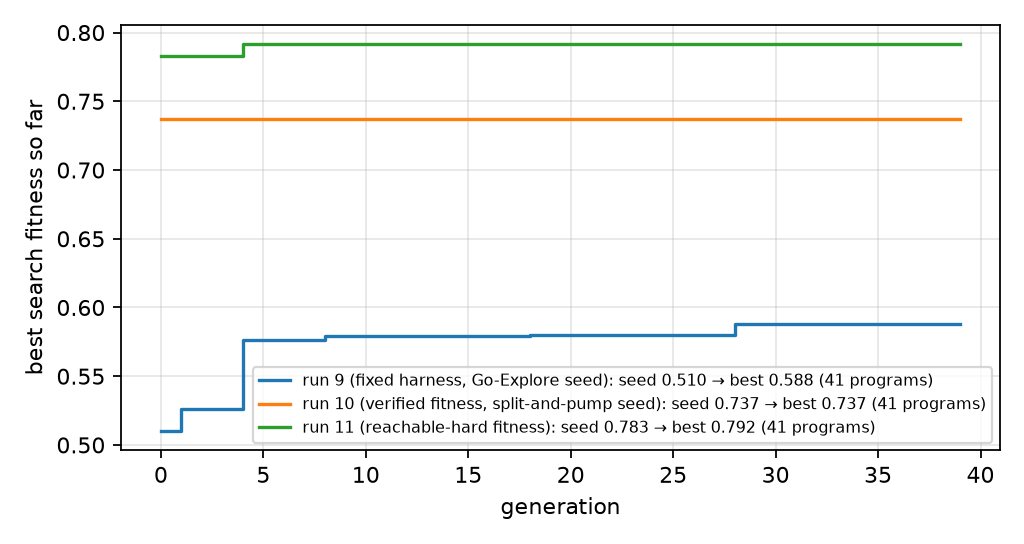
\includegraphics[width=0.52\linewidth]{figures/search_runs_fixed.png}
\caption{Best search fitness by generation on the fixed harness (each run on its own fitness scale). Run 9 (Go-Explore seed) climbs 0.510 $\to$ 0.588; run 10 (verified fitness, split-and-pump seed) never leaves generation 0; run 11 (reachable-hard fitness, same seed) makes its one gain at generation 4 (0.783 $\to$ 0.792) --- the gain that transfers (\S1.3). Every run finds whatever it finds within the first generations.}
\label{fig:fitness}\end{figure}


\section*{Part 3 --- Reflections}
% Reflections (<= 1 page). Post-reset draft by the agent; the author should rewrite in their own voice.
\subsection*{What this project suggests about autonomous ML research}
\textbf{A loop that scores itself will find the evaluator's cheapest defect.} Our loop found a race in its own archive within a few
generations and built a strategy around it; the transfer test, the ablations, the tuning study and the portfolios all confirmed the gain,
because all of them ran through the same evaluator. Nothing inside the loop could have told it apart from a discovery. The check that
caught it was the one that did not go through the evaluator: reproducing a concrete artefact --- an action chain --- from a level reset.
We now think every autonomous-research claim needs at least one such check, and that it should be part of the fitness, not a
post-hoc audit: once the replay was built into the score, the exploit became worthless to the search by construction.

\textbf{The ledger is the unit of disclosure, and the human's questions were its most useful rows.} The human posed the problem, set
constraints and approved compute; the agent did the rest. The interventions that mattered were not technical: ``are you planning or
reacting?'', ``what did we believe, what do we believe now?'', ``stop plugging leaks and build the ship''. Each produced a
structural change (a plan before GPU-hours; a claims table with before/after; verified fitness, invariants and a frozen protocol).
We suggest venues ask for the timestamped ledger rather than a binary autonomy label, and that authors quote the interventions.

\textbf{Negative results are cheap for an agent and expensive for a field.} The agent wrote and benchmarked 24 exploration
procedures in a night; most of the value was in the ones that failed the same way, because that is what showed the residual to be a
common barrier rather than a diversity problem. An autonomous loop makes this kind of exhaustive negative sweep affordable; the
discipline it needs is a frozen protocol, so that the sweep measures the procedures and not the drift of the evaluator.

\textbf{Compute was cheap; judgment was not.} The GPU-hours went to searches, benches and re-evaluations; the human hours went to
deciding what the headline could honestly be. The workshop's thesis --- autonomous research, human judgment --- was, for us,
literally the division of labor, and the judgment call that mattered most was withdrawing a result.


\bibliographystyle{plainnat}
\bibliography{refs}
\end{document}
